% enaR: Tools for Ecological Network Analysis
% Target: Methods in Ecology and Evolution
% October 2013
% ---------------------------------------------------
\documentclass[11pt]{article}
\usepackage[super, sort]{natbib}
  \bibpunct{(}{)}{;}{a}{,}{,} % required for natbib
\bibliographystyle{mee}

\usepackage[margin=1in]{geometry}

\usepackage{amsmath,amssymb,amsthm,amsfonts}
\usepackage[]{graphicx}
\usepackage{setspace} 
\usepackage{lineno} %numbers lines
\usepackage{qtree} %draw tree structures
\usepackage{url}

% --- SRB Defined functions ----
\newcommand{\ppr}{\lambda_1(\mathbf{A})}
\newcommand{\ID}{I/D}
\newcommand{\g}{\lambda_1(\mathbf{G})}
\DeclareMathOperator{\diag}{diag}
\def\citeapos#1{\citeauthor{#1}'s (\citeyear{#1})}
\newcommand{\R}{R}
%\newcommand{\S}{S}
\newcommand{\enaR}{\texttt{enaR}}
\newcommand{\vnorm}[1]{\left|\left|#1\right|\right|}
\newcommand{\midtilde}{\raisebox{-0.25\baselineskip}{\textasciitilde}}
\def\tableline{\vskip .1in \hrule height 0.6pt \vskip 0.1in}
% ----------------
\usepackage[ pdfauthor={Stuart R. Borrett},
pdfkeywords={ecological network analysis, network environ analysis},
pdfpagemode=UseOutlines, bookmarks=T, colorlinks,
linkcolor=blue,citecolor=blue, pdfstartview=FitH,
urlcolor=red]{hyperref}

% ---- FRONT MATTER -----

\title{\enaR: An \R\ package for Ecological Network Analysis}
\author{Stuart R. Borrett$^{a,*}$ and Matthew K. Lau$^b$
  \\ {\footnotesize $^a$ Department of Biology and Marine Biology,
    University of North Carolina Wilmington, Wilmington, NC, 28403}
  \\ {\footnotesize $^b$ Department of Biological Sciences and the
    Merriam-Powell Center for Environmental Research, Northern Arizona
    University, 617 S.\ Beaver St., Flagstaff, AZ, 86011}
  \\ {\footnotesize $^*$ Corresponding author, borretts@uncw.edu} }

% ------------------------
\begin{document}

%%%%%%%%%%%%%%%%%
%%%Title Page
%%%%%%%%%

\begin{description}
  \item[\textbf{Title}:] \enaR: An \R\ package for Ecological Network Analysis
  \item[\textbf{Running Title}:] R ecological network analysis package 
  \item[\textbf{Word Count}:] 3025
  \item[\textbf{Authors}:] Stuart R. Borrett, Matthew K. Lau
  \item[\textbf{Addresses}:] \
    \begin{itemize}
    \item SRB: Department of Biology and Marine Biology, University of
      North Carolina Wilmington, Wilmington, NC, 28403
    \item MKL: Department of Biological Sciences and the
      Merriam-Powell Center for Environmental Research, Northern
      Arizona University, 617 S. Beaver St., Flagstaff, AZ, 86011
    \end{itemize}
  \item[\textbf{Contact Details}:] \
    \begin{itemize}
    \item Email: borretts@uncw.edu
    \item Phone: 910.962.2411
    \item Fax: 910.962.4066
    \end{itemize}
\end{description}

\pagebreak

\maketitle

\begin{spacing}{2}
\linenumbers

\tableline
\section*{Abstract}
\begin{itemize}
\item Technological developments are making the collection of complex,
  relational datasets more common, a network approach is becoming an
  essential analytical method. Ecological Network Analysis (ENA) is an
  approach rooted in ecosystem ecology with over 30 years of
  development that investigates the structure, function, and evolution
  of ecological systems.
\item Here, we introduce \enaR , an \R\ package that enables
  ecologists to perform a broad set of ENA algorithms to analyze the
  structure and dynamics of ecosystem network models that quantify
  flows of energy or matter between discrete ecological compartments
  (e.g., food webs).
\item In addition to describing the primary functionality of the
  package, we also highlight several value added features, including a
  library of 100 empirical ecosystem models, the ability to analyze
  multiple models simultaneously, and connections to other analytical
  tools in \R .
\end{itemize}

KEYWORDS: network analysis, ecosystem, social network analysis,
software, network environ analysis, ascendency, input--output
analysis, food web, Ecopath, WAND
\tableline

\section{Introduction}
% Network Ecology & its significance
Network Ecology -- the study of ecological systems using network
models and analyses to characterize their structure, function, and
evolution -- is a large and rapidly growing area of ecology.
\citet{borrett14_rise} found that more than 5\% of the ecology and
evolutionary biology papers published in 2012 and indexed by Web of
Science could be classified as Network Ecology.  Likewise,
\citet{ings2009} showed that a notable fraction of 2008 publications
in 11 select journals were related to food webs ($\approx$2.4\%),
mutualistic networks ($\approx$0.9\%), and host-parasitoid networks
($\approx$0.055\%).  Network ecology is growing in part because
ecology is fundamentally a relational science and network models are
excellent tools for relational analyses.  In addition, the rise of
network ecology contributes to, mirrors, and builds on the more
general development of network sciences \citep{wasserman94,
%  barabasi02, 
barabasi12, borgatti2003network, freeman2004development,
  newman03review}

% what is ENA
Ecological Network Analysis (ENA) is a branch of network ecology that
is rooted in ecosystem ecology \citep{borrett12_netecol}.  It functions
as a ``macroscope'' to investigate (1) whole system organization,
(2) the direct and indirect effects among system components, and (3)
the processes that create and sustain ecological systems.  More
specifically, ENA is a family of algorithms that are an ecological
application and extension of the economic Input-Output Analysis
developed by Leontief (\citeyear{leontief66}).  These algorithms are
applied to network models of energy and matter exchange among
ecosystem components with the iconic example of this being the
food-web \citep{patten76, ulanowicz86, fath99_review, hannon73}.

% examples of recent use
The development of ENA has contributed to a new theoretical
understanding of ecosystems \citep{ulanowicz86, higashi91, belgrano05,
  jorgensen07_newecology} and the techniques have been applied in a
multiple ways.  For example, \citet{patten82} used a storage analysis
to identify two nearly separate hydrologic subsystems in the
Okefenokee Swamp, USA.  \citet{bondavalli99} showed that in the
Florida Everglades the American alligator is an indirect mutualist
with several of its prey, including frogs.  \citet{hines12} used
ENA to study the Cape Fear River estuary sediment nitrogen cycle, and applied
the tools to quantify the coupling between biogeochemical processes
(e.g., nitrification + anammox).  
%Subsequent work showed the potential
%impact of sea water intrusion on the N cycle \citep{hines14}. % this
                                % hines text is clunky.  Furthermore,
several scientists have used ENA to investigate urban sustainability
\citep{bodini02, zhang10_ecomod, chen12, bodini2012cities}.
Collectively, this work consistently shows the power of a network
approach to reveal patterns that are only evident at the scale of
entire systems \citep{ulanowicz90, patten91, fath07_netconstruction}.

% Objectives
We have created \enaR\ to provide open-source access to ENA tools.  We
had three specific design objectives for this software.  The first
objective was to collect the major ENA functions into a single
software package, which we describe below.  The second was to increase
both the availability and extensibility of the software. We chose to
implement the software in \R\ because of its increasing popularity as
an analytical tool in the biological sciences
\citep[e.g.,][]{dixon2003vegan, metcalf2012, revell2012phytools}.
Users can freely download a stable version of the package from the
CRAN website (\url{http://cran.r-project.org/web/packages/enaR/}), and
development is being conducted via GitHub
(\url{https://github.com/TheSeeLab/enaR}).  The third design objective
was to let users connect to other analytical tools.  To enable this,
\enaR\ was built specifically to connect to two existing \R\ network
analysis packages:  \texttt{network} \citep{butts08_network} and
\texttt{sna} \citep{butts08_social}.  In summary, the aim of the
\enaR\ package is to make ENA tools more available and easier to use,
adapt, and extend.  In this paper, we present \enaR  with a brief
illustration of its functionality. For a more detailed user
introduction, please refer to the package vignette: \url{http://cran.r-project.org/web/packages/enaR/vignettes/enaR.pdf}.

\section{Overview of \enaR}
ENA was devleoped to analyze network models of energy or matter flow
and storage in an ecosystem.  More generally, the analyses could be
used to analyze any system in which some physically conserved unit
moves among compartments. After describing the data required as
input to ENA, we highlight the primary ENA algorithms currently
included in \enaR\ .  We then walk through an application of the
\enaR\ Flow analysis to an example ecosystem model.

\subsection{Data Requirements and Input}
% ENA Data requirements and Input -- no math
For ENA, the system is modeled as a set of compartments or network nodes that
represent species, species-complexes (i.e., trophic guilds or
functional groups), or non-living components of the system in which
energy or matter is stored.  These nodes are connected by a set of
observed fluxes, termed directed edges or links.  %The estimates of the
%internal system energy--matter flow from $i$ to $j$ are notated as
%$\mathbf{F}_{n\times n}=[f_{ij}]$, $i,j=1,2,\ldots,n$. 
These models also have energy--matter inputs into the system
%$\mathbf{z}_{1 \times n}=[z_i]$
 and output losses from the system.
%$\mathbf{y}_{1 \times n}=[y_i]$. 
The full set of data required to perform ENA includes: (1) internal
flows, (2) boundary inputs, (3) boundary exports, (4) boundary
respiration, (5) boundary outputs, which may be the sum of exports and
respiration, (6) biomass or storage values, and (7) designation of
living status of each node.

As ENA is an agglomeration of tools developed by multiple perspectives
\citep[e.g.,][]{patten59, margalef63, hannon73, pimm82,
  golley1993history}, the data requirements vary from function to
function. The main differences arise from two distinct schools of
thought that have driven the development of ENA since the 1970s
\citep{scharler09comparing}.  The first school is based on the work of
Dr.\ Robert E. Ulanowicz and colleagues at the University of Maryland
\citep{ulanowicz86, ulanowicz97, ulanowicz09_window}.  Primarily
focused on trophic ecology, this approach uses information theory and
the ascendency concept that characterizes ecosystem growth and
development \citet{ulanowicz86, ulanowicz97}.  The second school is
based on the work of Dr.\ Bernard C. Patten at the University of
Georgia \citep{patten76, matis81, patten82, fath99_review}.  Steeped
in dynamic equations, simulations, and systems analysis, this work
developed the environ concept that formalizes the concept of
environment \citep{patten78} and has often been referred to as
``Network Environ Analysis.'' 

The primary difference in data requirements among ENA functions is
that the Patten School treats all outputs the same, while the
Ulanowicz School partitions outputs into respiration
%$\mathbf{r}_{1\times
%  n}=[r_i]$ 
and export 
%$\mathbf{e}_{1\times n}=[e_i]$ 
to account for differences in energetic quality between these two
types of ecosystem output. Note that the more
generic outputs can be the sum of the respiration and export values.
%$y_i = r_i + e_i$ for all $i$.  
The final required information is a categorization of each node as
living or not, which is essential for algorithms from the Ulanowicz
School.  We specified this node attribute by creating a logical vector
%$\mathbf{Living}_{1 \times n}$ 
that indicates whether the %$i^{th}$ 
node is living (TRUE) or not (FALSE). Some analyses also need the amount of energy--matter stored
in each node (e.g., biomass).%, $\mathbf{X}_{1\times n}=[x_i]$.

% % ENA Data requirements and Input
% For ENA, the system is modeled as a set of $n$ compartments or nodes
% that represent species, species-complexes (i.e., trophic guilds or
% functional groups), or non-living components of the system in which
% energy or matter is stored.  These nodes are connected by $L$ observed
% fluxes, termed directed edges or links.  The estimates of the internal
% system energy--matter flow from $i$ to $j$ are notated as
% $\mathbf{F}_{n\times n}=[f_{ij}]$, $i,j=1,2,\ldots,n$.  These models
% also have energy--matter inputs into the system $\mathbf{z}_{1 \times
%   n}=[z_i]$, and output losses from the system $\mathbf{y}_{1 \times
%   n}=[y_i]$.  While the Patten School treats all outputs the same, the
% Ulanowicz School partitions outputs into respiration
% $\mathbf{r}_{1\times n}=[r_i]$ and export $\mathbf{e}_{1\times
%   n}=[e_i]$ to account for differences in energetic quality. Note that
% $y_i = r_i + e_i$ for all $i$.  Some analyses also need the amount of
% energy--matter stored in each node (e.g., biomass),
% $\mathbf{X}_{1\times n}=[x_i]$.  The final required information is a
% categorization of each node as living or not, which is essential for
% algorithms from the Ulanowicz School.  We specified this node
% attribute by creating a logical vector $\mathbf{Living}_{1 \times n}$
% that indicates whether the $i^{th}$ node is living (TRUE) or not
% (FALSE).  Together, the model data can be summarized as $\{\mathbf{F},
% \mathbf{z}, \mathbf{e}, \mathbf{r}, \mathbf{X}, \mathbf{Living}\}$.

%% THOUGHT 10-14-2013 -- given that the paper does not introduce the
%% mathematics, perhaps we should leave out the mathematical formalism
%% here.  This might make the paper more readable for a general
%% audience.

Most analytical functions in \enaR\ assume the model data is presented
as an \R\ network data object defined in the \texttt{network} package.
Given the data elements, the \texttt{pack} function can be used to
manually combine the data elements to create the necessary \R\ network
data object. While there is no standard data format for an ENA model,
there are two commonly used formats.  First, there is the Scientific
Committee for Ocean Research (SCOR) format that is the required input
to NETWRK \citep{ulanowicz91}, and the second format is the Excel sheet
formatted data that is the input to WAND \citep{allesina04_wand}.  The
\enaR\ package includes a \texttt{read.scor} and a \texttt{read.wand}
function to read in these common data formats.

\subsection{Included Algorithms}
% enaR Algorithms
Although not comprehensive, the package currently includes many of the
most commonly used algorithms (Table~\ref{tab:alg}), along with a
number of work flow tools (e.g., the ``read'' functions mentioned
above).  \enaR\ captures all of the Patten School algorithms
previously implemented in NEA.m, along with some recent developments.
Ulanowicz School algorithms are more limited, including the ascendency
calculations \citep{ulanowicz97} and mixed trophic impacts analyses
\citep{ulanowicz90}.  It is our hope that user participation will
develop the the package further through the inclusion of more
algorithms.

\subsection{Example Application}
% Apply enaR to a single model.
Given a network model, applying ENA algorithms with \enaR\ is straight
forward. Although the functions vary in their specifications and the
results that are returned to the user, all \enaR\ functions follow a
similar argument structure.  All analytical functions begin with the
prefix 'ena' followed by the specific analysis name (see
Table~\ref{tab:alg}). For simplicity's sake, we demonstrate how to use
the package with an example that conducts Flow analysis on a published
ecosystem model. Table~\ref{tab:flow} shows an example script for
applying the ENA Flow analysis to the six compartment model of energy
flow in the South Carolina oyster reef ecosystem
\citep{dame81}. Briefly, the analysis invovles: (1) loading the model
data, (2) checking and balancing the model if necessary, and (3)
inputing the balanced model into the analysis function.

After loading the \enaR\ package, the first step is to enter the model
data.  In this example, we use the \texttt{read.scor} function to import
the SCOR formatted data from a text file.  We can then apply one of
four automated balancing algorithms introduced by \citet[AVG,
  Input-Output, Output-Input, AVG2,][]{allesina03} to ensure that the
model is at steady-state --- one of the assumptions of the flow
analysis.  In this example we used the default AVG2 algorithm, which
tends to cause the least distortion of flows while balancing the
network \citep{allesina03}.  We then apply the \texttt{enaFlow}
function to the model to perform the desired ENA flow analysis.  This
analysis returns 4 matrices ($\mathbf{G}$, $\mathbf{GP}$,
$\mathbf{N}$, $\mathbf{NP}$) and two vectors (throughflow, $T$, and a
vector of 20 whole-network statistics, $ns$).  Guidance for how to
interpret these results can be found in previously published
literature \citep{fath06, schramski11}.

\subsection{Visualization}
% Visualization
Visualization of network models can be an essential analytical tool
\citep{moody05dynamic,lima2011visual}.  Because \enaR\ is built on top
of the \texttt{network} package and data type, it is possible to
quickly create network plots of the model internal structure.
Fig.~\ref{fig:example}a shows an example of the Oyster Reef ecosystem
model.  The \texttt{network} package includes three network layout
algorithms: circle, Fruchterman-Reingold, and Kamada-Kawai.  The
Fruchterman-Reingold algorithm used here is the default.
% mention lack of cross boundary input/output?

\section{Value Added Features}
Beyond the basic functionality of the \enaR\ package, there are
several features that add substantive value for users.  We highlight
three of these features here: the ecosystem model library, multiole
model or ``batch'' analysis, and connections to other network analysis
tools.

\subsection{Model Library}
% Model Library
To facilitate new systems ecology and network science, we included a
library of 100 previously published ecosystem network models with the
\enaR\ package. These models each trace a thermodynamically conserved
unit (e.g., C, N, P) through a particular ecosystem.  The models in
this set are empirically-based in that the authors attempted to model
a specific system and parameterized the model to some degree with
empirical estimates.  The library includes models used previously to
test several systems ecology hypotheses \citep{borrett10_idd,
  borrett10_hmg, salas11_did, borrett13}.  This set has a 47\%
overlap with the set of models previously collected by Dr.\ Ulanowicz
(\url{http://www.cbl.umces.edu/~ulan/ntwk/network.html}).

We have tentatively split these models into two classes.  The most
abundant class is the trophic network models. % (Table~\ref{tab:TRO}).
These models tend to have a food web at their core, but also include
non-trophic fluxes generated by processes like death and excretion.
The annual carbon flux model for the mesohaline region of the
Chesapeake Bay is a typical example \citep{baird89}.  The second class
of models focuses on biogeochemical cycling.  % (Table~\ref{tab:BGC}).
In contrast to the trophic networks, the biogeochemical cycling models
tend to have more highly aggregated nodes (more species grouped into a
compartment), include more abiotic nodes that could represent chemical
species (e.g., ammonia in a nitrogen cycle), have a lower dissipation
rate, and therefore they tend to have more recycling
\citep{christian96, borrett10_idd}.  \citeapos{christian03} models of
nitrogen cycling in the Neuse River Estuary are good examples of the
class.  The package vignette has a full listing of the models included
along with references to their original publications \citep{enar}.

\subsection{Batch Analysis}
Major advancements in ecosystem ecology have been made through an
approach that examines network metric for multiple ecosystem
models. For example, \citet{christensen95} applied ENA to identify and
compare the maturity of 41 ecosystem models,
%\citet{hines14} used a comparative approach to
%investigate the impact of sea level rise on process coupling in the
%estuarine nitrogen cycle. 
\citet{baird08_sylt} compared different nutrient dynamics in the
Sylt-R{\o}m{\o} Bight ecosystem, and \citet{vanoevelen2011canyon}
compared the food webs and their organic matter processing in three
sections of the Nazar{\'e} submarine canyon.  The \enaR\ tool
simplifies the work flow for these types of comparison. Given a list
of models like the model library, it is possible to quickly analyze
multiple models using R's \texttt{lapply} function (see
\texttt{help}(``lapply'')).  This facilitates the kind of comparative
network analysis often of interest to ecologists
\citep{monaco97,christian05_cnea}.
% I could use examples from ECOMOD special issue.

Batch analysis can be used in several additional ways.  One
application is for meta-analyses, such as tests of the generality of
hypothesized ecosystem properties like network non-locality
\citep{salas11_did}, %and network homogenization
\citep{borrett10_hmg}, or to investigate how physical features might
influence ENA results
\citep{niquil2012physical}. Fig.~\ref{fig:example}b illustrates the
rank-ordered network homogenization statistic for the 56 trophic-based
ecosystem models in the library. Notice that the homogenization
statistic is greater than one in all of these models indicating that
the network of indirect interactions tend to more uniformly distribute
the resources than is obvious from the direct interactions, which
extends previous results of \citet{borrett10_hmg} to include several
new models.  A second kind of application is the exploration of new
ENA inter-relationships.  Given the collection of the Patten and
Ulanowicz school algorithms and the library of models, the ENA
community can investigate possible relationships among the ENA
indicators from different schools (Fig.~\ref{fig:example}c).  A third
application of batch analysis is to investigate the previously unknown
empirical ranges of ENA whole-network statistics, which may be useful
for interpreting results from specific applications.
Fig.~\ref{fig:ns} shows the observed distribution of values for
selected network statistics from the 100 models in the library easily
analyzed using \texttt{lapply} and the associated \enaR\ functions.

\subsection{New Connections}
% Connections to other tools (SNA, igraph)
A fourth key feature of the \enaR\ package design is that it enables
network ecologists easier access to other network tools and analyses
that might be useful.  The \enaR\ package uses the \R\ network data
structure defined in the \texttt{network} package
\citep{butts08_network}.  This means that network ecologists using \enaR\
can also use the network manipulation functions and visualization
features of the \texttt{network} package. Further, the \R\ Social
Network Analysis (SNA) package, \texttt{sna}, \citep{butts08_social} also uses this
network data object.  This means that network ecologists can apply
many of the SNA algorithms directly to their ecological network
models.  For example, Fig.~\ref{fig:example}d illustrates applying the betweenness
centrality function to the Chesapeake Bay trophic model
\citep{baird89} and visualizing the results using the target
centrality plot \citep{brandes03}.  This analysis highlights the
central role of Sedimentary Particulate Carbon and bacteria in the
Sediment Particulate Organic Carbon (POC) in the carbon flux of the
estuary.

In addition, \enaR\ can be a starting point for ecosystem network
ecologists to use other \R\ network tools.  For example, the
\texttt{iGraph} package provides functions to apply classic graph
theory \citep{csardi06}.  The \texttt{limSolve} package provides
capabilities to infer network model fluxes from empirical data by
linear inverse modeling \citep{soetaert09}, which can also be used for
uncertainty analyses of ENA \citep{kones09}. There are a wealth of
additional \R\ package that network ecologists may find useful
including \texttt{bipartite} \citep{dormann2008}, \texttt{vegan}
\citep{dixon2003vegan}, \texttt{bioconductor}
\citep{gentleman2004bioconductor}, \texttt{Cheddar}
\citep{hudson2013}, \texttt{Diversitree} \citep{fitzjohn2012}, and
packages in the \texttt{statnet} family \citep{handcock2008statnet}
beyond \texttt{network} and \texttt{sna}.

\section{Conclusion and Future Development}
% Existing Software/Tools : NETWRK, WAND, ECOPATH, NEA.m EcoNet
Several software tools have been created to previously to enable
scientists to apply ENA. The first widely distributed tool was NETWRK
\citep{ulanowicz91}.  This program is a collection of analyses
programmed in Fortran and distributed as a DOS executable
file. Version 4.2 is available from
%(\href{http://www.cbl.umces.edu/~ulan/ntwk/network.html}{http://www.cbl.umces.edu/$\sim$ulan/ntwk/network.html}).
\url{http://www.cbl.umces.edu/~ulan/ntwk/network.html}. WAND is a
Microsoft Excel based re-implementation of many but not all of the
algorithms in NETWRK \citep{allesina04_wand}. An explicit goal of WAND
was to be more accessible for ecologists, who have tended to be more
familiar with Excel than DOS.  \citet{fath06} introduced a Matlab
function, NEA.m, which collected algorithms largely developed for
network environ enalysis, hence NEA \citep{patten91}.  One advantage
of NEA.m is that the algorithms are transparent to the user and
accessible for modification.  While the NEA.m function is freely
available
(\url{http://www.mathworks.com/matlabcentral/fileexchange/5261-nea-m})
%{http://www.mathworks.com/matlabcentral/fileexchange/5261-nea-m})
it requires Matlab, which is powerful but expensive proprietary
software.  With modification, the function can be run in Octave, an
open source clone of Matlab, but it executes more slowly and doesn't
have the same level of support provided by Matlab.  EcoNet is a
web-based tool that lets users apply ENA analyses similar to to NEA.m,
but with some computational enhancements \citep{kazanci07,
  schramski11}.  Ecopath with Ecosim \citep{christensen92,
  christensen04} is used primarily for model construction and
simulation, but it also includes a network analysis plug-in that
implements several other ENA algorithms.  Other tools have been
created, but do not appear to have a large user base
\citep{latham2006,kones09}. A challenge for ENA users has been that no
existing software covers all of the major analyses, which has lead to
separate, over-lapping approaches to ENA and high variation in
software availability, usability, and extensibility.

The \enaR\ package addresses many of the limitations of the previously
published set of ENA tools. The library joins analyses from both the
currently separate schools of ENA into a single software package.
The library is built in \R\ so that the functions are transparent and
adaptable by the community of users.  It also lets users have access
to other network and statistical analysis tools that are already part
of \R. 
%
In the future, we anticipate two initial lines of continued
development for the \enaR\ package. The first is to increase the
connections between the \enaR\ package and other modeling and
analytical tools.  For example, we are currently working with
colleagues to enable users of Ecopath with Ecosim
\citep{christensen04} to apply the \enaR\ tools in a seamless way.  We
are also developing functions to connect between \enaR\ and the
\R\ limSolve package \citep{soetaert09} for creating models using
Linear Inverse Modeling and to enable uncertainty analysis
\citep{kones09}.

The second line of development is to extend the package's
capabilities.  While it currently contains most of the many commonly
used ENA algorithms used by ecologists, it is far from complete. For
example, \citeapos{ulanowicz83} decomposition of cycles is not yet
included nor is his construction for the Lindeman trophic spine
\citep{ulanowicz1979trophic}. The package could also include network
model construction tools, such as least-inference methods for building
models from empirical data \citep{ulanowicz2008least} and
\citeapos{fath04_cyber} algorithm for constructing plausible
ecosystems models.
%
Looking to the future of ENA, we hope to facilitate the rapid
developemnt of accessible network analysis tools for the ecological
community. A major reason for our use of open source software is that
we want to foster user driven development and extension of the
package's functionality. Although the network approach promotes
innovation and collaboration across fields, network ecology has
developed along multiple, largely separate lines
\citep{scharler09comparing,allesina2012}.  It is our hope that
\enaR\ can serve as an organizing point for ENA and other ecological
network methods with the hope that doing so will not only produce
relevant software, but also promote feedback bewteen theory and
applications. Toward this end, we have developed the GitHub
development repository
(\url{https://github.com/MKLau/enaR_development}) and project page
(\url{http://theseelab.github.io/enaR/}), where researchers can find
more information on how to contribute software. Together, the
open-source tools for vasersion control and project management
provided by Git and GitHub will increase the potential for
collaborative software development. We look forward to working with
the dynamic community of peoople interested in network analyses to
promote the use and development of network tools in ecology.

\section{Acknowledgments}
We would like to acknowledge and thank David Hines for contributing to
the initial code.  We also thank several individuals who used the
earlier versions of the software and provided helpful feedback for
further development including Ursula Scharler, Shaoqing Chen, Emily
Oxe, and John Mejaski.  In addition, we thank the many ecosystem model
authors who created, shared, and published their work.  This work was
funded in part by the US National Science Foundation (DEB1020944,
DEB0425908), an NSF Integrative Graduate Education and Research
Traineeship (MKL; DGE0549505) and a UNCW Cahill award (SRB).

\end{spacing}
%%%%%%%%%%%%%%%%%%%%%%%%%%%%%%%%%%%%%%%%%%%%%%%%%%%%%%%%%%%%%%%%%%%%%%%%%%%%%%%
%\section{Bibliography}
%\bibliography{/Users/borretts/research/srbbib_abb,/Users/borretts/research/srb}
\begin{thebibliography}{79}
\providecommand{\natexlab}[1]{#1}

\bibitem[{Allesina \& Bondavalli(2003)}]{allesina03}
Allesina, S. \& Bondavalli, C. (2003) Steady state of ecosystem flow networks:
  A comparison between balancing procedures.
\newblock \emph{Ecol Model}, \textbf{165}, 221--229.

\bibitem[{Allesina \& Bondavalli(2004)}]{allesina04_wand}
Allesina, S. \& Bondavalli, C. (2004) Wand: An ecological network analysis
  user-friendly tool.
\newblock \emph{Environ Model Softw}, \textbf{19}, 337--340.

\bibitem[{Allesina (2012)}]{allesina2012}
Allesina, S. (2012) Ecology: The more the merrier.
\newblock \emph{Nature}, \textbf{487}, 175--176.

\bibitem[{Baird \emph{et~al.}(2008)Baird, Asmus \& Asmus}]{baird08_sylt}
Baird, D., Asmus, H. \& Asmus, R. (2008) Nutrient dynamics in the
  {S}ylt-{R}{\o}m{\o} {B}ight ecosystem, {German Wadden Sea}: An ecological
  network analysis approach.
\newblock \emph{Estuar Coast Shelf Sci}, \textbf{80}, 339--356.

\bibitem[{Baird \& Ulanowicz(1989)}]{baird89}
Baird, D. \& Ulanowicz, R.E. (1989) The seasonal dynamics of the {Chesapeake
  Bay} ecosystem.
\newblock \emph{Ecol Monogr}, \textbf{59}, 329--364.

\bibitem[{Barab{\'a}si(2012)}]{barabasi12}
Barab{\'a}si, A.L. (2012) The network takeover.
\newblock \emph{Nature Physics}, \textbf{8}, 14--16.

\bibitem[{Belgrano \emph{et~al.}(2005)Belgrano, Scharler, Dunne \&
  Ulanowicz}]{belgrano05}
Belgrano, A., Scharler, U.M., Dunne, J. \& Ulanowicz, R.E. (2005) \emph{Aquatic
  Food Webs: An Ecosystem Approach}.
\newblock Oxford University Press, New York, NY.

\bibitem[{Bodini \& Bondavalli(2002)}]{bodini02}
Bodini, A. \& Bondavalli, C. (2002) Towards a sustainable use of water
  resources: a whole-ecosystem approach using network analysis.
\newblock \emph{Int J Environmental Pollution}, \textbf{18}, 463--485.

\bibitem[{Bodini \emph{et~al.}(2012)Bodini, Bondavalli \&
  Allesina}]{bodini2012cities}
Bodini, A., Bondavalli, C. \& Allesina, S. (2012) Cities as ecosystems: Growth,
  development and implications for sustainability.
\newblock \emph{Ecol Model}, \textbf{245}, 185--198.

\bibitem[{Bondavalli \& Ulanowicz(1999)}]{bondavalli99}
Bondavalli, C. \& Ulanowicz, R.E. (1999) Unexpected effects of predators upon
  their prey: {T}he case of the {A}merican alligator.
\newblock \emph{Ecosystems}, \textbf{2}, 49--63.

\bibitem[{Borgatti \& Foster(2003)}]{borgatti2003network}
Borgatti, S.P. \& Foster, P.C. (2003) The network paradigm in organizational
  research: A review and typology.
\newblock \emph{J Manage}, \textbf{29}, 991--1013.

\bibitem[{Borrett(2013)}]{borrett13}
Borrett, S.R. (2013) Throughflow centrality is a global indicator of the
  functional importance of species in ecosystems.
\newblock \emph{Ecol Indic}, \textbf{32}, 182--196.

\bibitem[{Borrett \emph{et~al.}(2012)Borrett, Christian \&
  Ulanowicz}]{borrett12_netecol}
Borrett, S.R., Christian, R.R. \& Ulanowicz, R.E. (2012) Network ecology.
\newblock A.H. El-Shaarawi \& W.W. Piegorsch, eds., \emph{Encyclopedia of
  Environmetrics}, pp. 1767--1772. John Wiley \& Sons, 2nd edition.

\bibitem[{Borrett \emph{et~al.}(submitted)Borrett, Moody \&
  Edelmann}]{borrett14_rise}
Borrett, S.R., Moody, J. \& Edelmann, A. (submitted) The rise of network
  ecology: maps of the topic diversity and scientific collaboration.
\newblock \emph{Ecol Model}.

\bibitem[{Borrett \& Salas(2010)}]{borrett10_hmg}
Borrett, S.R. \& Salas, A.K. (2010) Evidence for resource homogenization in 50
  trophic ecosystem networks.
\newblock \emph{Ecol Model}, \textbf{221}, 1710--1716.

\bibitem[{Borrett \emph{et~al.}(2010)Borrett, Whipple \&
  Patten}]{borrett10_idd}
Borrett, S.R., Whipple, S.J. \& Patten, B.C. (2010) Rapid development of
  indirect effects in ecological networks.
\newblock \emph{Oikos}, \textbf{119}, 1136--1148.

\bibitem[{Brandes \emph{et~al.}(2003)Brandes, Kenis \& Wagner}]{brandes03}
Brandes, U., Kenis, P. \& Wagner, D. (2003) Communicating centrality in policy
  network drawings.
\newblock \emph{IEEE Transactions on Visualization and Computer Graphics},
  \textbf{9}, 241--253.

\bibitem[{Butts(2008{\natexlab{a}})}]{butts08_network}
Butts, C. (2008{\natexlab{a}}) network: A package for managing relational data
  in {R}.
\newblock \emph{J Stat Softw}, \textbf{24}.

\bibitem[{Butts(2008{\natexlab{b}})}]{butts08_social}
Butts, C. (2008{\natexlab{b}}) Social network analysis with sna.
\newblock \emph{J Stat Softw}, \textbf{24}, 1--51.

\bibitem[{Chen \& Chen(2012)}]{chen12}
Chen, S. \& Chen, B. (2012) Network environ perspective for urban metabolism
  and carbon emissions: A case study of {Vienna, A}ustria.
\newblock \emph{Environ Sci Tech}, \textbf{46}, 4498--4506.

\bibitem[{Christensen(1995)}]{christensen95}
Christensen, V. (1995) Ecosystem maturity---towards quantification.
\newblock \emph{Ecol Model}, \textbf{77}, 3--32.

\bibitem[{Christensen \& Pauly(1992)}]{christensen92}
Christensen, V. \& Pauly, D. (1992) Ecopath-{II}---a software for balancing
  steady-state ecosystem models and calculating network characteristics.
\newblock \emph{Ecol Model}, \textbf{61}, 169--185.

\bibitem[{Christensen \& Walters(2004)}]{christensen04}
Christensen, V. \& Walters, C.J. (2004) Ecopath with {E}cosim: {M}ethods,
  capabilities and limitations.
\newblock \emph{Ecol Model}, \textbf{172}, 109--139.

\bibitem[{Christian \emph{et~al.}(2005)Christian, Baird, Luczkovich, Johnson,
  Scharler \& Ulanowicz}]{christian05_cnea}
Christian, R.R., Baird, D., Luczkovich, J., Johnson, J.C., Scharler, U.M. \&
  Ulanowicz, R.E. (2005) Role of network analysis in comparative ecosystem
  ecology of estuaries.
\newblock A.~Belgrano, J.~Scharler U. M.~Dunne \& R.~Ulanowicz, eds.,
  \emph{Aquatic Food Webs: An Ecosystem Approach}, pp. 25--40. Oxford
  University Press, New York, NY.

\bibitem[{Christian \emph{et~al.}(1996)Christian, Fores, Comin, Viaroli, Naldi
  \& Ferrari}]{christian96}
Christian, R.R., Fores, E., Comin, F., Viaroli, P., Naldi, M. \& Ferrari, I.
  (1996) Nitrogen cycling networks of coastal ecosystems: influence of trophic
  status and primary producer form.
\newblock \emph{Ecol Model}, \textbf{87}, 111--129.

\bibitem[{Christian \& Thomas(2003)}]{christian03}
Christian, R.R. \& Thomas, C.R. (2003) Network analysis of nitrogen inputs and
  cycling in the {Neuse River Estuary, North Carolina, USA}.
\newblock \emph{Estuaries}, \textbf{26}, 815--828.

\bibitem[{Csardi \& Nepusz(2006)}]{csardi06}
Csardi, G. \& Nepusz, T. (2006) The igraph software package for complex network
  research.
\newblock \emph{InterJournal}, \textbf{Complex Systems}, 1695.

\bibitem[{Dame \& Patten(1981)}]{dame81}
Dame, R.F. \& Patten, B.C. (1981) Analysis of energy flows in an intertidal
  oyster reef.
\newblock \emph{Mar Ecol Prog Ser}, \textbf{5}, 115--124.

\bibitem[{Dixon(2003)}]{dixon2003vegan}
Dixon, P. (2003) {VEGAN}, a package of {R} functions for community ecology.
\newblock \emph{Journal of Vegetation Science}, \textbf{14}, 927--930.

\bibitem[{Dormann \emph{et~al.}(2008)Dormann, Gruber \& Fr{\"u}nd}]{dormann2008}
Dormann, C.F., Gruber, B. \& Fr{\"u}nd, J. (2008) Introducing the bipartite
  package: analysing ecological networks.
\newblock \emph{\R\ News}, \textbf{8}, 8--11.

\bibitem[{Fath(2004)}]{fath04_cyber}
Fath, B.D. (2004) Network analysis applied to large-scale cyber-ecosystems.
\newblock \emph{Ecol Model}, \textbf{171}, 329--337.

\bibitem[{Fath \& Borrett(2006)}]{fath06}
Fath, B.D. \& Borrett, S.R. (2006) A {Matlab}\copyright\ function for network
  environ analysis.
\newblock \emph{Environ Model Softw}, \textbf{21}, 375--405.

\bibitem[{Fath \& Patten(1999)}]{fath99_review}
Fath, B.D. \& Patten, B.C. (1999) Review of the foundations of network environ
  analysis.
\newblock \emph{Ecosystems}, \textbf{2}, 167--179.

\bibitem[{Fath \emph{et~al.}(2007)Fath, Scharler, Ulanowicz \&
  Hannon}]{fath07_netconstruction}
Fath, B.D., Scharler, U.M., Ulanowicz, R.E. \& Hannon, B. (2007) Ecological
  network analysis: network construction.
\newblock \emph{Ecol Model}, \textbf{208}, 49--55.

\bibitem[{FitzJohn(2012)}]{fitzjohn2012}
FitzJohn, R.G. (2012) Diversitree: comparative phylogenetic analyses of
  diversification in {R}.
\newblock \emph{Methods Ecol Evol}, \textbf{3}, 1084--1092.

\bibitem[{Freeman(2004)}]{freeman2004development}
Freeman, L.C. (2004) \emph{The development of social network analysis: A study
  in the sociology of science}.
\newblock Empirical Press Vancouver.

\bibitem[{Gentleman \emph{et~al.}(2004)Gentleman, Carey, Bates, Bolstad,
  Dettling, Dudoit, Ellis, Gautier, Ge, Gentry
  \emph{et~al.}}]{gentleman2004bioconductor}
Gentleman, R.C., Carey, V.J., Bates, D.M., Bolstad, B., Dettling, M., Dudoit,
  S., Ellis, B., Gautier, L., Ge, Y., Gentry, J. \emph{et~al.} (2004)
  Bioconductor: open software development for computational biology and
  bioinformatics.
\newblock \emph{Genome biology}, \textbf{5}, R80.

\bibitem[{Golley(1993)}]{golley1993history}
Golley, F. (1993) \emph{A history of the ecosystem concept in ecology: More
  than the sum of the parts}.
\newblock Yale University Press, New Haven, CT.

\bibitem[{Handcock \emph{et~al.}(2008)Handcock, Hunter, Butts, Goodreau \&
  Morris}]{handcock2008statnet}
Handcock, M., Hunter, D., Butts, C., Goodreau, S. \& Morris, M. (2008) statnet:
  Software tools for the representation, visualization, analysis and simulation
  of network data.
\newblock \emph{J Stat Softw}, \textbf{24}, 1548.

\bibitem[{Hannon(1973)}]{hannon73}
Hannon, B. (1973) The structure of ecosystems.
\newblock \emph{J Theor Biol}, \textbf{41}, 535--546.

\bibitem[{Higashi \& Burns(1991)}]{higashi91}
Higashi, M. \& Burns, T.P. (1991) \emph{Theoretical studies of ecosystems: The
  network perspective}.
\newblock Cambridge University Press, Cambridge.

\bibitem[{Hines \emph{et~al.}(2012)Hines, Lisa, Song, Tobias \&
  Borrett}]{hines12}
Hines, D.E., Lisa, J.A., Song, B., Tobias, C.R. \& Borrett, S.R. (2012) A
  network model shows the importance of coupled processes in the microbial {N}
  cycle in the {Cape Fear River} estuary.
\newblock \emph{Estuar Coast Shelf Sci}, \textbf{106}, 45--57.

\bibitem[{Hudson \emph{et~al.}(2013)Hudson, Emerson, Jenkins, Layer, Ledger,
  Pichler, Thompson, O'Gorman, Woodward \& Reuman}]{hudson2013}
Hudson, L.N., Emerson, R., Jenkins, G.B., Layer, K., Ledger, M.E., Pichler,
  D.E., Thompson, M.S.A., O'Gorman, E.J., Woodward, G. \& Reuman, D.C. (2013)
  Cheddar: analysis and visualisation of ecological communities in {R}.
\newblock \emph{Methods Ecol Evol}, \textbf{4}, 99--104.

\bibitem[{Ings \emph{et~al.}(2009)Ings, Montoya, Bascompte, Bl{\"u}thgen,
  Brown, Dormann, Edwards, Figueroa, Jacob, Jones, Lauridsen, Ledger, Lewis,
  Olesen, van Veen \& Warren}]{ings2009}
Ings, T.C., Montoya, J.M., Bascompte, J., Bl{\"u}thgen, N., Brown, L., Dormann,
  C.F., Edwards, F., Figueroa, D., Jacob, U., Jones, J.I., Lauridsen, R.B.,
  Ledger, M.E., Lewis, H.M., Olesen, J.M., van Veen, F.J.F. \& Warren, P. H.
  nad~Woodward, G. (2009) Review: Ecological networks--beyond food webs.
\newblock \emph{J Anim Ecol}, \textbf{78}, 253--269.

\bibitem[{J{\o}rgensen \emph{et~al.}(2007)J{\o}rgensen, Fath, Bastianoni,
  Marques, M\"{u}ller, Nielsen, Patten, Tiezzi \&
  Ulanowicz}]{jorgensen07_newecology}
J{\o}rgensen, S.E., Fath, B.D., Bastianoni, S., Marques, J.C., M\"{u}ller, F.,
  Nielsen, S., Patten, B.C., Tiezzi, E. \& Ulanowicz, R.E. (2007) \emph{A new
  ecology: Systems perspective}.
\newblock Elsevier, Amsterdam.

\bibitem[{Kazanci(2007)}]{kazanci07}
Kazanci, C. (2007) Eco{N}et: A new software for ecological modeling, simulation
  and network analysis.
\newblock \emph{Ecol Model}, \textbf{208}, 3--8.

\bibitem[{Kones \emph{et~al.}(2009)Kones, Soetaert, van Oevelen \&
  Owino}]{kones09}
Kones, J.K., Soetaert, K., van Oevelen, D. \& Owino, J.O. (2009) Are network
  indices robust indicators of food web functioning? a {M}onte {C}arlo
  approach.
\newblock \emph{Ecol Model}, \textbf{220}, 370--382.

\bibitem[{Latham~II(2006)}]{latham2006}
Latham~II, L.G. (2006) Network flow analysis algorithms.
\newblock \emph{Ecol Model}, \textbf{192}, 586--600.

\bibitem[{Lau \emph{et~al.}(2013)Lau, Borrett \& Hines}]{enar}
Lau, M.K., Borrett, S.R. \& Hines, D.E. (2013) \emph{enaR: Tools for ecological
  network analysis in R}.
\newblock R package version 2.5.

\bibitem[{Leontief(1966)}]{leontief66}
Leontief, W.W. (1966) \emph{Input--Output Economics}.
\newblock Oxford University Press, New York.

\bibitem[{Lima(2011)}]{lima2011visual}
Lima, M. (2011) \emph{Visual complexity: mapping patterns of information}.
\newblock Princeton Architectural Press.

\bibitem[{Margalef(1963)}]{margalef63}
Margalef, R. (1963) Certain unifying principles in ecology.
\newblock \emph{Am Nat}, \textbf{97}, 357--374.

\bibitem[{Matis \& Patten(1981)}]{matis81}
Matis, J.H. \& Patten, B.C. (1981) Environ analysis of linear compartmental
  systems: the static, time invariant case.
\newblock \emph{Bull Int Stat Inst}, \textbf{48}, 527--565.

\bibitem[{Metcalf \emph{et~al.}(2012)Metcalf, McMahon, Salguero-G{\'o}mez \&
  Jongejans}]{metcalf2012}
Metcalf, C.J.E., McMahon, S.M., Salguero-G{\'o}mez, R. \& Jongejans, E. (2012)
  {IPM}pack: an {R} package for integral projection models.
\newblock \emph{Methods Ecol Evol}, \textbf{4}, 195--200.

\bibitem[{Monaco \& Ulanowicz(1997)}]{monaco97}
Monaco, M.E. \& Ulanowicz, R.E. (1997) Comparative ecosystem trophic structure
  of three us mid-{A}tlantic estuaries.
\newblock \emph{Mar Ecol Prog Ser}, \textbf{161}, 239--254.

\bibitem[{Moody \emph{et~al.}(2005)Moody, McFarland \&
  Bender-deMoll}]{moody05dynamic}
Moody, J., McFarland, D. \& Bender-deMoll, S. (2005) Dynamic network
  visualization.
\newblock \emph{American Journal of Sociology}, \textbf{110}, 1206--1241.

\bibitem[{Newman(2003)}]{newman03review}
Newman, M. (2003) The structure and function of complex networks.
\newblock \emph{SIAM review}, \textbf{45}, 167--256.

\bibitem[{Niquil \emph{et~al.}(2012)Niquil, Chaumillon, Johnson, Bertin, Grami,
  David, Bacher, Asmus, Baird \& Asmus}]{niquil2012physical}
Niquil, N., Chaumillon, E., Johnson, G., Bertin, X., Grami, B., David, V.,
  Bacher, C., Asmus, H., Baird, D. \& Asmus, R. (2012) The effect of physical
  drivers on ecosystem indices derived from ecological network analysis:
  Comparison across estuarine ecosystems.
\newblock \emph{Estuar Coast Shelf Sci}, \textbf{108}, 132--143.

\bibitem[{Patten(1959)}]{patten59}
Patten, B.C. (1959) An introduction to the cybernetics of the ecosystem: The
  trophic dynamic aspect.
\newblock \emph{Ecology}, \textbf{40}, 221---231.

\bibitem[{Patten(1978)}]{patten78}
Patten, B.C. (1978) Systems approach to the concept of environment.
\newblock \emph{Ohio J Sci}, \textbf{78}, 206--222.

\bibitem[{Patten(1982)}]{patten82}
Patten, B.C. (1982) Environs: Relativistic elementary particles for ecology.
\newblock \emph{Am Nat}, \textbf{119}, 179--219.

\bibitem[{Patten(1991)}]{patten91}
Patten, B.C. (1991) Network ecology: Indirect determination of the
  life--environment relationship in ecosystems.
\newblock M.~Higashi \& T.~Burns, eds., \emph{Theoretical Studies of
  Ecosystems: The Network Perspective}, pp. 288--351. Cambridge University
  Press, New York.

\bibitem[{Patten \emph{et~al.}(1976)Patten, Bosserman, Finn \& Cale}]{patten76}
Patten, B.C., Bosserman, R.W., Finn, J.T. \& Cale, W.G. (1976) Propagation of
  cause in ecosystems.
\newblock B.C. Patten, ed., \emph{Systems Analysis and Simulation in Ecology,
  Vol. IV}, pp. 457--579. Academic Press, New York.

\bibitem[{Pimm(1982)}]{pimm82}
Pimm, S.L. (1982) \emph{Food webs}.
\newblock Chapman and Hall, London; New York.

\bibitem[{Revell(2012)}]{revell2012phytools}
Revell, L.J. (2012) phytools: an {R} package for phylogenetic comparative
  biology (and other things).
\newblock \emph{Methods Ecol Evol}, \textbf{3}, 217--223.

\bibitem[{Salas \& Borrett(2011)}]{salas11_did}
Salas, A.K. \& Borrett, S.R. (2011) Evidence for dominance of indirect effects
  in 50 trophic ecosystem networks.
\newblock \emph{Ecol Model}, \textbf{222}, 1192--1204.

\bibitem[{Scharler \& Fath(2009)}]{scharler09comparing}
Scharler, U. \& Fath, B. (2009) Comparing network analysis methodologies for
  consumer--resource relations at species and ecosystems scales.
\newblock \emph{Ecol Model}, \textbf{220}, 3210--3218.

\bibitem[{Schramski \emph{et~al.}(2011)Schramski, Kazanci \&
  Tollner}]{schramski11}
Schramski, J.R., Kazanci, C. \& Tollner, E.W. (2011) Network environ theory,
  simulation and {EcoNet}\copyright\ 2.0.
\newblock \emph{Environ Model Softw}, \textbf{26}, 419--428.

\bibitem[{Soetaert \emph{et~al.}(2009)Soetaert, Van~den Meersche \& van
  Oevelen}]{soetaert09}
Soetaert, K., Van~den Meersche, K. \& van Oevelen, D. (2009) \emph{limSolve:
  Solving Linear Inverse Models}.
\newblock R package version 1.5.1.

\bibitem[{Ulanowicz(1983)}]{ulanowicz83}
Ulanowicz, R.E. (1983) Identifying the structure of cycling in ecosystems.
\newblock \emph{Math Biosci}, \textbf{65}, 219--237.

\bibitem[{Ulanowicz(1986)}]{ulanowicz86}
Ulanowicz, R.E. (1986) \emph{Growth and Development: Ecosystems Phenomenology}.
\newblock Springer--Verlag, New York.

\bibitem[{Ulanowicz(1997)}]{ulanowicz97}
Ulanowicz, R.E. (1997) \emph{Ecology, the Ascendent Perspective}.
\newblock Columbia University Press, New York.

\bibitem[{Ulanowicz(2009)}]{ulanowicz09_window}
Ulanowicz, R.E. (2009) \emph{A third window, {N}atural life beyond {N}ewton and
  {D}arwin}.
\newblock Templeton Foundation Press, West Conshohocken, PA.

\bibitem[{Ulanowicz \& Kay(1991)}]{ulanowicz91}
Ulanowicz, R.E. \& Kay, J. (1991) A package for the analysis of ecosystem flow
  networks.
\newblock \emph{Environmental Software}, \textbf{6}, 131--142.

\bibitem[{Ulanowicz \& Kemp(1979)}]{ulanowicz1979trophic}
Ulanowicz, R.E. \& Kemp, W.M. (1979) Toward canonical trophic aggregations.
\newblock \emph{Am Nat}, \textbf{114}, 871--883.

\bibitem[{Ulanowicz \& Puccia(1990)}]{ulanowicz90}
Ulanowicz, R.E. \& Puccia, C.J. (1990) Mixed trophic impacts in ecosystems.
\newblock \emph{Coenoses}, \textbf{5}, 7--16.

\bibitem[{Ulanowicz \& Scharler(2008)}]{ulanowicz2008least}
Ulanowicz, R.E. \& Scharler, U.M. (2008) Least-inference methods for
  constructing networks of trophic flows.
\newblock \emph{Ecol Model}, \textbf{210}, 278--286.

\bibitem[{van Oevelen \emph{et~al.}(2011)van Oevelen, Soetaert, Garc{\'\i}a,
  de~Stigter, Cunha, Pusceddu \& Danovaro}]{vanoevelen2011canyon}
van Oevelen, D., Soetaert, K., Garc{\'\i}a, R., de~Stigter, H.C., Cunha, M.R.,
  Pusceddu, A. \& Danovaro, R. (2011) Canyon conditions impact carbon flows in
  food webs of three sections of the nazar{\'e} canyon.
\newblock \emph{Deep-Sea Res Pt II}, \textbf{58}, 2461--2476.

\bibitem[{Wasserman \& Faust(1994)}]{wasserman94}
Wasserman, S. \& Faust, K. (1994) \emph{Social network analysis: {M}ethods and
  applications}.
\newblock Cambridge University Press, Cambridge; New York.

\bibitem[{Zhang \emph{et~al.}(2010)Zhang, Yang, Fath \& Li}]{zhang10_ecomod}
Zhang, Y., Yang, Z.F., Fath, B.D. \& Li, S.S. (2010) Ecological network
  analysis of an urban energy metabolic system: Model development, and a case
  study of four {C}hinese cities.
\newblock \emph{Ecol Model}, \textbf{221}, 1865--1879.

\end{thebibliography}



%\listoffigures

%\listoftables

\clearpage
\newpage
% ========================================================================================
\section{Tables}
%% TABLE: Primary Algorithms/Functions
\begin{table*}[h]
\center
\caption{Primary Ecological Network Analysis algorithms in \enaR.}\label{tab:alg}
\tableline
%\begin{scriptsize}
\begin{tabular}{l l l l l }
\textbf{Analysis} & \textbf{Function Name} & \textbf{School} \\ \hline \\ [1.5ex]
Structure & \texttt{enaStructure} & foundational, Patten \\
Flow & \texttt{enaFlow} & foundational, Patten \\
Ascendency & \texttt{enaAscendency} & Ulanowicz \\
Storage & \texttt{enaStorage} & Patten \\
Utility & \texttt{enaUtility} & Patten \\
Mixed Trophic Impacts & \texttt{enaMTI} & Ulanowicz \\
Control & \texttt{enaControl} & Patten \\
Environ & \texttt{enaEnviron} & Patten \\
\end{tabular}
%\end{scriptsize}
\tableline
\end{table*}

\newpage
\begin{table*}
\center
\caption{Example code for applying \enaR\ Flow analysis to \citeapos{dame81} oyster
  reef model.} \label{tab:flow}
\tableline
\begin{verbatim}
> library(enaR)                 # load package
> m <- read.scor("oyster.dat")  # read model data from SCOR formatted file
> m <- balance(m)               # balance model using AVG2 algorithm 
[1] BALANCED
> u <- unpack(m)                # unpack model data to illustrate components
> attributes(u)
$names
[1] "F"      "z"      "r"      "e"      "y"      "X"      "Living"

> F <- enaFlow(m)               # perform ENA flow analysis
> attributes(F)                  # show analysis objects created
$names
[1] "T"  "G"  "GP" "N"  "NP" "ns"

> F$ns                          # show flow analysis network statistics
     Boundary     TST     TSTp      APL       FCI       BFI       DFI       IFI
[1,]    41.47 83.5833 125.0533 2.015512 0.1101686 0.4961517 0.1950689 0.3087794
         ID.F   ID.F.I   ID.F.O    HMG.I    HMG.O AMP.I AMP.O mode0.F  mode1.F
[1,] 1.582925 1.716607 1.534181 2.051826 1.891638     3     1   41.47 32.90504
      mode2.F  mode3.F mode4.F
[1,] 9.208256 32.90504   41.47
> 
\end{verbatim}

\tableline
\end{table*}

\clearpage
\newpage

% ========================================================================================
\section{Figures}

\begin{figure*}[h]
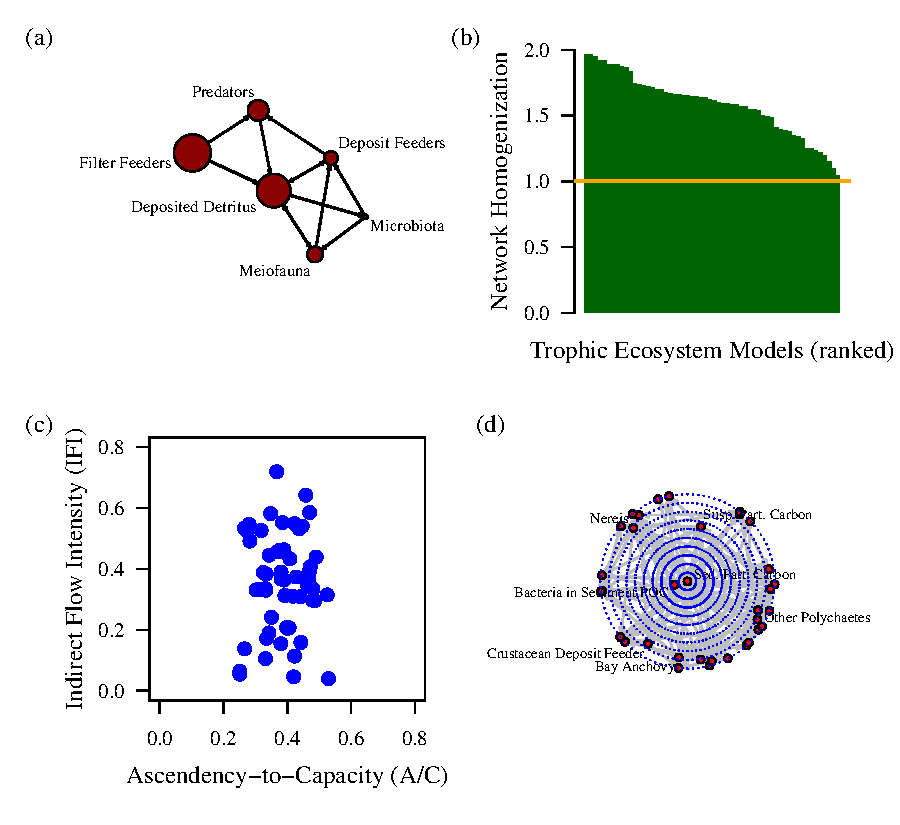
\includegraphics[scale=1]{../figures/enaR_plot_example.pdf}
\caption{Example of analysis and visualizations created with \enaR\:
  (a) network digraph of the internal flows of an oyster reef
  ecosystem model \citep{dame81}, (b) network homogenization statistic
  for 56 trophic ecosystem models (rank-ordered), (c) scatter plot
  showing the relationship between the ascendency-to-capacity ratio
  and the indirect flow index for the 56 trophic ecosystem models
  (Table~xx), and (d) target plot of the betweenness centrality from
  social network analysis calculated for the xx nodes of the
  Chesapeake Bay ecosystem model \citep{baird89}. } \label{fig:example}
\end{figure*}

\begin{figure*}[t]
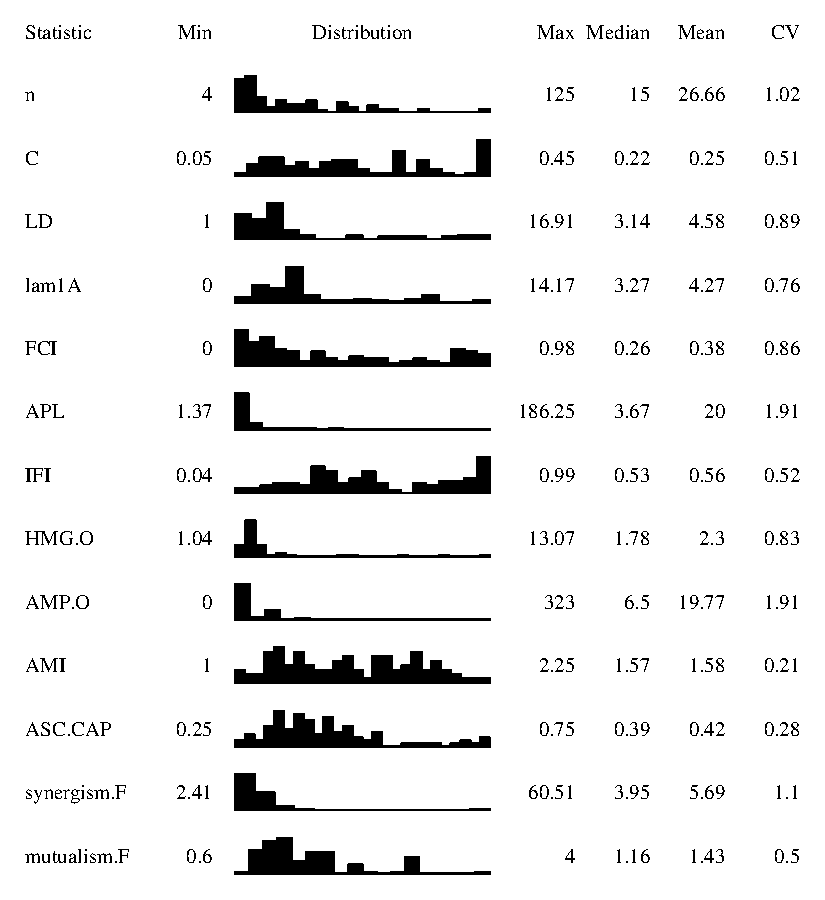
\includegraphics[scale=1]{../figures/ns_dist.pdf}
\caption{Distributions of selected ENA network statistics from to the
  100 empirically-based ecosystem models included in \enaR.  The
  results are summarized using a histogram showing the distribution of
  the values of each network statistic between the observed minimum
  and maximum values.  The median, mean, and coefficient of variation
  (ratio of standard deviation and mean) values are also reported.
  The network statistics are the number of nodes ($n$), the
  connectance ($C = L/n^2$), link density ($LD = L/n$), pathway
  proliferation rate (lam1A), Finn cycling index (FCI), average path
  length (APL), indirect flow intensity (IFI), output oriented network
  homogenization ratio (HMG.O), output-oriented network amplification
  ratio (AMP.O), average mutual information (AMI), the
  ascendency-to-capacity ratio (ASC.CAP), flow-based network synergism
  (synergism.F) and mutualism (mutualism.F).} \label{fig:ns}
\end{figure*}

\end{document}
